% Single-contract dynamics on hourly candles. Every number traces to data/research/pm_vol/*.json
% (written by src/albert/research/pm_vol.py) or to report research-pm-vol-20261109T215533Z.

We begin with the stylized facts and then document each one. Throughout, ``estimation sample''
means steps that end before 1 October 2026 and ``holdout'' means October 2026.
\begin{enumerate}
\item Where the sample is broad, prices behave as calibrated martingales with the fixed total
  variance that M0 implies.
\item The information clock depends strongly on the category. In-game sports follow the uniform
  clock $\irate=1/\tauexp$ almost exactly. Pre-game sports run at a few per cent of that rate, and
  weather information is concentrated in the last day.
\item Outside in-game sports, increments are far from Gaussian. Most hours show no mid change, and
  most of the variance arrives in jumps.
\item The backbone lies between Jacobi ($\beta=1/2$) and probit. Logit-normal ($\beta=1$) is
  rejected.
\item Stochastic volatility beyond the clock is present but short-lived. Filtering it improves
  variance forecasts under QLIKE but not under MSE.
\end{enumerate}

\subsubsection{Martingale property and the variance identity}\label{sec:dyn-res-mart}

For a calibrated martingale, the sum of squared price changes over a contract's life plus the final
move to settlement has the same expectation as $\pr_0(1-\pr_0)$ (\cref{sec:model}).
\Cref{tab:dyn-vi} in \cref{app:dyn} reports the ratio of the two by category.
% source: data/research/pm_vol/results_vi.json:variance_identity (sample_h = 6)
Weather and sports, the two categories sampled broadly, satisfy the identity. Sampled
  every six hours, the ratio is 0.97 (estimation sample) and 0.93 (holdout) for weather, on 5{,}838
  and 4{,}595 markets. For sports it is 0.98 and 1.01, on 9{,}533 and 10{,}007 markets.
Calibration alone, $\E(y-\pr_0)^2/\E\,\pr_0(1-\pr_0)$, is 0.96 and 0.94 for weather and
  0.99 and 1.01 for sports.
The smaller categories show ratios of 1.0--1.6. Their candle samples were partly
  selected by trading volume, which is ex post, so they over-represent markets that moved. We
  therefore do not read these ratios as evidence against the martingale.

Over six-hour horizons, the mean mid change conditional on the price bin,
  $\E[\pr_{t+6\text{h}}-\pr_t\mid\pr_t]$, has $|t|<2$ in 129 of 156 category-by-split-by-bin cells.
  The 17 cells with a mean of at least 0.3\cents{} and $|t|\ge2$ have mixed signs and no common
  location in $\pr$.
  % source: data/research/pm_vol/maker.json:martingale

\subsubsection{Information clocks}\label{sec:dyn-res-clock}

\Cref{tab:dyn-clock} summarizes the clock fits and \cref{fig:dyn-clock} plots the piecewise
information rate against the uniform clock.
In-game sports are the one regime in which M0 holds in level and shape. With the
  uniform clock to the scheduled end, $\Var(\ustd)$ is 1.02 in the estimation sample and 1.02 in the
  holdout, and excess kurtosis is 3--4. No alternative clock improves the holdout likelihood by more
  than 0.004 nats per step. This is the Brownian game model of \citet{stern1994} observed in prices.

Pre-game sports resolve information at about 4\% of the uniform rate (scaled clock,
  $a=0.04$), and the rate rises steeply in the last hours before the start. Under the uniform clock
  $\Var(\ustd)$ is 0.09 in the holdout. The bucket clock with an hour-of-day profile improves the
  holdout likelihood by 1.24 nats per step ($t=8.9$).
Weather concentrates information in the final day, with $\irate\propto\tauexp^{-2.8}$
  and an hour-of-day profile; the gain over uniform is 0.16 nats per step ($t=10.8$).

Mentions, Politics and Entertainment track the uniform clock in level beyond about a
  day. On the estimation sample their gains come mainly from the hour-of-day profile: Politics gains
  0.198 nats per step with it and 0.043 without.
In Politics, Entertainment and Science \& Technology the clock
  chosen on the estimation sample does not beat the uniform clock on the holdout. October volatility
  there was 1.3--2.3 times the fitted clock ($\Var(\ustd)$ of 1.26--2.31).
% source: data/research/pm_vol/results_cat.json:categories.*.clock_table, clock_fits

\begin{table}[t]
\centering
\begin{threeparttable}
\caption{Information clocks by category}\label{tab:dyn-clock}
\scriptsize
\setlength{\tabcolsep}{2.5pt}
% source: data/research/pm_vol/results_cat.json:categories.*.{n_dev,n_holdout,events_*,clock_chosen,clock_fits,clock_table,u_diag}
\begin{tabular}{lccccccccc}
\toprule
 & Steps & Events & Clock & \multicolumn{2}{c}{Shape} & $\Delta$NLL & \multicolumn{2}{c}{$\Var(\ustd)$} & Exc.\ kurt. \\
\cmidrule(lr){5-6}\cmidrule(lr){8-9}
Category & est.\ / holdout & est.\ / hold. & (BIC) & $a$ & $b$ & vs.\ uniform ($t$) & uniform & fitted & fitted \\
\midrule
Sports in-game & 11{,}536 / 9{,}448 & 5371 / 4488 & Power & 0.97 & 0.86 & 0.004 (5.4) & 1.02 & 1.03 & 3 \\
Sports pre-game & 473{,}272 / 252{,}089 & 8137 / 6014 & Buckets$\times$hour & 0.04 & 5.75 & 1.241 (8.9) & 0.09 & 1.30 & 618 \\
Weather & 102{,}284 / 64{,}657 & 1189 / 840 & Power$\times$hour & 0.98 & 2.81 & 0.163 (10.8) & 0.88 & 1.03 & 22 \\
Mentions & 35{,}261 / 15{,}888 & 105 / 59 & Buckets$\times$hour & 0.85 & 1.10 & 0.114 (1.9) & 0.76 & 1.07 & 582 \\
Politics & 39{,}941 / 21{,}891 & 120 / 100 & Power$\times$hour & 1.12 & 0.72 & $-0.059$ ($-0.3$) & 0.48 & 1.28 & 1281 \\
Elections & 103{,}634 / 0 & 95 / 0 & Power$\times$hour & 1.13 & 0.98 & -- & 1.13$^\dagger$ & 1.00$^\dagger$ & 205$^\dagger$ \\
Entertainment & 199{,}724 / 29{,}501 & 182 / 64 & Buckets$\times$hour & 0.71 & 0.87 & 0.025 (0.2) & 0.74 & 1.26 & 542 \\
Sci.\ \& Tech. & 29{,}154 / 8{,}251 & 90 / 79 & Buckets$\times$hour & 1.27 & 0.80 & $-0.093$ ($-1.0$) & 1.95 & 2.31 & 59 \\
\bottomrule
\end{tabular}
\begin{tablenotes}[flushleft]\footnotesize
\item Hourly steps; decision quote spread $\le4$\cents{} and mid in $[0.03,0.97]$. Estimation sample: steps ending before 1 October 2026; holdout: October 2026.
\item \emph{Clock}: form with the lowest BIC on the estimation sample. \emph{Shape}: $a$ of the scaled clock $\irate=a/\tauexp$ and $b$ of the power clock $\irate=a\tauexp^{-b}$ (uniform: $a=b=1$).
\item $\Delta$NLL: holdout mean negative log-likelihood per step of the uniform clock minus that of the chosen clock (positive: the chosen clock fits better), $t$ clustered by event.
\item $\Var(\ustd)$ and excess kurtosis of \cref{eq:dyn-u} on the holdout. $^\dagger$Elections has no holdout (\cref{sec:dyn-sample}); estimation-sample values.
\end{tablenotes}
\end{threeparttable}
\end{table}

\begin{figure}[t]
\centering
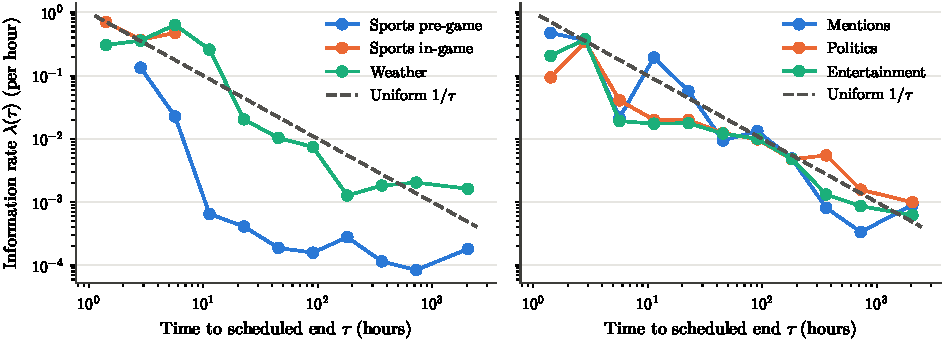
\includegraphics[width=\textwidth]{figures/fig_dyn_clock.pdf}
\caption{Information rate $\irate(\tauexp)$ per hour from the piecewise-constant clock fitted on the estimation sample (before 1 October 2026), against time to the scheduled end of information. The dashed line is the uniform clock $1/\tauexp$; buckets without data are omitted. In-game sports sit on the uniform clock; pre-game sports run one to two orders of magnitude below it; weather information is front-loaded into the final day.}
\label{fig:dyn-clock}
\end{figure}

\subsubsection{Distribution of innovations and jumps}\label{sec:dyn-res-shape}

\Cref{fig:dyn-u} contrasts the variance and the shape of $\ustd$. Once the clock is fitted,
$\Var(\ustd)$ is close to one by construction on the estimation sample. The shape, however, is far
from Gaussian everywhere except in-game.

Holdout excess kurtosis is 22 for weather and 59--1281 in the other non-sports
  categories and pre-game sports. With the fitted clock, $P(|\ustd|>4)$ is 0.7--2.7\% against
  0.006\% for a normal.
  % source: results_cat.json:categories.*.u_diag
Outside in-game sports (12\%), the mid does not change in 22\%
  (weather) to 85\% (Elections) of hours.
The EM mixture assigns 55--85\% of $\sum(\Delta\pr)^2$ to the jump
  component, with similar values in the estimation sample and the holdout (\cref{tab:dyn-sv}).
Outside in-game sports, the probability that a
  $|\ustd|>3$ hour is followed by another is 4.5--15\%, against an unconditional 1.4--4.7\%. Large moves cluster only mildly, so the
  tails are mainly isolated jumps rather than prolonged high-volatility episodes.
  % source: results_cat.json:categories.*.jumps.{big_after_big,big_uncond}

This matters for anyone using the model as a density. For contracts more than seven days from
their scheduled end in Mentions, Politics, Elections, Entertainment and Science \& Technology, the
Gaussian M0 overstates the mean one-hour $|\Delta\pr|$ by a factor of 2.1--3.4 across price groups.
The M2 mixture, which includes the zero-move mass, gives 0.7--1.2 times the realized value. Closer
to expiry, and for sports and weather, the two bracket the realized move.
% source: data/research/pm_vol/maker.json:economic (tau group >7d)

\begin{figure}[t]
\centering
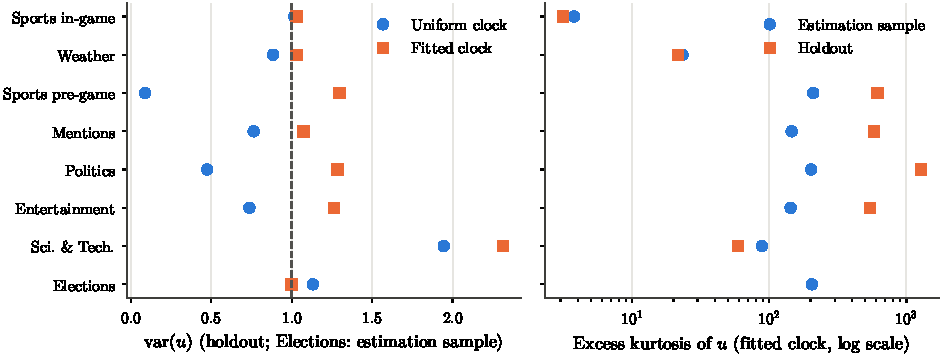
\includegraphics[width=\textwidth]{figures/fig_dyn_u.pdf}
\caption{Standardized innovations $\ustd$ (\cref{eq:dyn-u}) by category. Left: holdout (October 2026) variance under the uniform and the fitted clock; Elections has no holdout and shows the estimation sample. Right: excess kurtosis under the fitted clock, estimation sample and holdout, on a log scale. Only in-game sports are close to Gaussian.}
\label{fig:dyn-u}
\end{figure}

\subsubsection{Backbone}\label{sec:dyn-res-backbone}

\Cref{fig:dyn-backbone} plots squared price changes against the price level, after removing the
clock and quote noise.
Variance falls toward the edges more slowly than the probit backbone of M0
  implies, and far more slowly than the logit-normal backbone $[\pr(1-\pr)]^2$.
The QLIKE estimate of $\beta$ is 0.39 for pre-game sports, 0.47
  in-game, 0.58 for weather and 0.31--0.81 elsewhere. The Roll-corrected cell regression gives 0.44,
  0.49 and 0.54 for the same three categories in the estimation sample (\cref{tab:dyn-backbone}).

Logit-normal is rejected. It loses to probit on the estimation sample in every
  category ($t$ from 3.5 to 7.8, except Elections at 1.0). On the holdout it is worse in six of seven
  categories, significantly so in three (in-game $t=4.7$, weather $2.8$, Politics $2.4$).
Out of sample, the free-$\beta$ backbone beats probit in pre-game sports
  ($t=-1.7$), in-game ($-2.5$) and weather ($-1.8$), and loses in Entertainment ($+1.6$).
% source: results_cat.json:categories.*.backbone_table, beta_cells

Part of the extra volatility near the edges reflects the 1\cents{} tick: at $\pr=0.04$ a one-tick
move is large relative to $\varphi(\Phi^{-1}(\pr))$. The tick-grid control of
\cref{sec:dyn-res-drift} shows how much the grid alone distorts probit-unit statistics.

\begin{figure}[t]
\centering
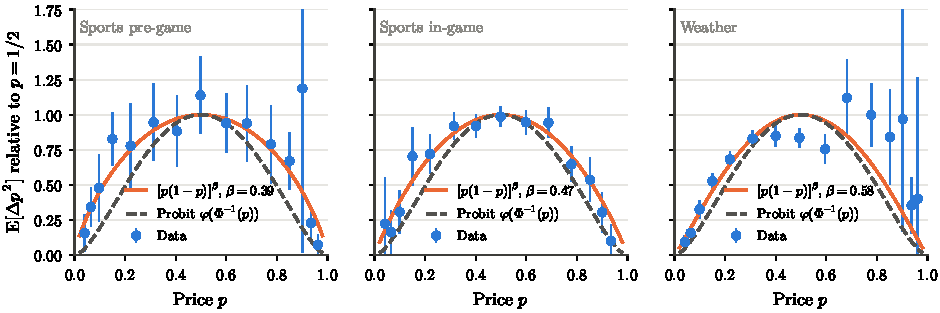
\includegraphics[width=\textwidth]{figures/fig_dyn_backbone.pdf}
\caption{Backbone. Points: mean of $[(\Delta \pr)^2-k s^2]/c_{j(\tauexp)}^2$ by price bin, estimation sample (before 1 October 2026), with $\pm2$ event-clustered standard errors; $c_j$ and $k$ are from the fitted power backbone, so the series is normalized to one at $\pr=1/2$. The solid line is the fitted $[\pr(1-\pr)]^{2\beta}$, normalized the same way; the dashed line is the probit backbone $\varphi(\Phi^{-1}(\pr))^2$ of M0. The logit-normal curve ($\beta=1$) lies below both and is omitted.}
\label{fig:dyn-backbone}
\end{figure}

\subsubsection{Stochastic volatility and leverage}\label{sec:dyn-res-sv}

\Cref{tab:dyn-sv} reports volatility clustering after the fitted clock is removed.
The within-market first-order autocorrelation of $|\ustd|$, which nets out
  static differences in volatility between markets, is 0.09--0.14 on the estimation sample ($t$ from
  2.0 to 6.4). It remains positive on the holdout, at 0.06--0.30.

The within-market half-life is 7--21 hours. The implied M1 vol-of-vol
  $\nu$ is 0.29--0.48 per $\sqrt{\text{day}}$. Weather is the exception, at 40 hours: its markets
  mostly live under 48 hours, so the within-market estimate rests on few markets.
Outside weather, the pooled autocorrelation decays more
  slowly, with half-lives of 21--29 hours; the difference is persistent heterogeneity in $\alpha$
  across markets.
% source: results_cat.json:categories.*.sv.{dev,holdout}.{acf_chosen,acf_within,fit_within,leverage,leverage_price_space}

The vol--price correlation $\rho$ is robust only in-game.
In-game, volatility rises after moves toward $1/2$: the correlation is $-0.11$
  ($t=-7.0$) on the estimation sample and $-0.08$ ($t=-4.2$) on the holdout in probit units, and
  $-0.14$ ($t=-8.8$) in price units.
Elsewhere the probit-unit correlation is indistinguishable from zero, except
  Entertainment and Science \& Technology ($+0.02$ and $+0.06$, $t\approx3$). The price-unit
  correlation is small and negative (weather $-0.03$, $t=-5.7$).
Because the sign depends on the units outside the in-game regime, we attribute it there to
backbone and tick mechanics rather than to a structural $\rho$. \Cref{sec:res-hf} shows that the
in-game effect is absent at minute scales.

\begin{table}[t]
\centering
\begin{threeparttable}
\caption{Stochastic volatility, leverage and jumps}\label{tab:dyn-sv}
\scriptsize
\setlength{\tabcolsep}{2.2pt}
% source: data/research/pm_vol/results_cat.json:categories.*.sv, jumps
\begin{tabular}{lccccccccc}
\toprule
 & \multicolumn{3}{c}{$\Corr(|\ustd_t|,|\ustd_{t+1}|)$} & Half-life & $\nu$ & \multicolumn{2}{c}{Leverage corr.\ ($t$)} & Jump share & Zero- \\
\cmidrule(lr){2-4}\cmidrule(lr){7-8}
Category & pooled & within ($t$) & within, hold. & (h) & per $\sqrt{\text{day}}$ & probit & price & est.\ / hold. & move \\
\midrule
Sports in-game & 0.12 & -- & 0.22 & -- & -- & $-0.109$ ($-7.0$) & $-0.144$ ($-8.8$) & 0.66 / 0.65 & 0.12 \\
Sports pre-game & 0.16 & 0.14 (6.4) & 0.21 & 9.4 & 0.48 & 0.001 (0.2) & $-0.009$ ($-2.2$) & 0.74 / 0.72 & 0.73 \\
Weather & 0.13 & 0.12 (2.0) & 0.30 & 40.1 & 0.16 & $-0.010$ ($-1.7$) & $-0.034$ ($-5.7$) & 0.62 / 0.55 & 0.22 \\
Mentions & 0.09 & 0.09 (5.5) & 0.06 & 6.8 & 0.44 & 0.006 (0.6) & $-0.003$ ($-0.3$) & 0.85 / 0.82 & 0.72 \\
Politics & 0.11 & 0.09 (4.6) & 0.28 & 11.6 & 0.33 & 0.009 (0.7) & $-0.031$ ($-2.4$) & 0.78 / 0.85 & 0.76 \\
Elections & 0.13 & 0.13 (3.5) & -- & 21.2 & 0.29 & $-0.001$ ($-0.1$) & $-0.023$ ($-1.5$) & 0.81 / -- & 0.85 \\
Entertainment & 0.11 & 0.09 (5.9) & 0.12 & 13.4 & 0.33 & 0.022 (3.2) & 0.006 (0.8) & 0.70 / 0.73 & 0.81 \\
Sci.\ \& Tech. & 0.14 & 0.10 (4.4) & 0.24 & 11.6 & 0.40 & 0.059 (3.5) & 0.021 (1.5) & 0.76 / 0.80 & 0.72 \\
\bottomrule
\end{tabular}
\begin{tablenotes}[flushleft]\footnotesize
\item Hourly $\ustd$ under the fitted clock. Estimation sample: before 1 October 2026; holdout: October 2026. Unless marked, statistics are from the estimation sample.
\item \emph{Within}: $|\ustd|$ demeaned by market, markets with at least 48 steps (in-game legs are too short). Half-life and $\nu$ come from the within-market fit $A\phi^k$, $k=1,\ldots,24$ (\cref{sec:dyn-sv}).
\item \emph{Leverage}: $\Corr(\sgn(\Zt_t)x_t,\,\tfrac16\sum_{j\le6}|x_{t+j}|)$ for $\pr\in[0.1,0.9]$, with $x=\ustd$ (probit) or $x=\Delta\pr$ over the backbone volatility (price); negative means volatility rises after moves toward $1/2$.
\item \emph{Jump share}: posterior-weighted share of $\sum(\Delta\pr)^2$ from the EM jump component (\cref{eq:dyn-em}). \emph{Zero-move}: share of hours without a mid change.
\item $t$ clustered by event.
\end{tablenotes}
\end{threeparttable}
\end{table}

\subsubsection{Forecasting realized variance}\label{sec:dyn-res-forecast}

\Cref{tab:dyn-forecast} compares the forecasts on the holdout.
Under QLIKE, M1 (fitted clock with the filtered
  vol state) beats \textsc{hist} in pre-game sports (one hour: $t=-6.0$; six hours: $t=-30.3$),
  weather ($-8.2$ and $-6.1$), in-game sports ($-3.0$) and Politics at one hour ($-2.2$).
The filtered state improves on M0 without it in pre-game
  sports ($t=-2.8$ and $-2.2$), in-game ($-3.1$), Politics at one hour ($-5.2$) and Mentions at six
  hours ($-2.2$).
M1 does not beat \textsc{hist} for Mentions, the category whose
  scheduled end drifts by about ten hours in October.

QLIKE and MSE disagree. Under MSE, M1 is never significantly better than M0 and is
  significantly worse in several cases (pre-game sports: $t=2.3$ and $4.2$). Down-weighting a quiet
  market pays under QLIKE, which penalizes under-prediction of small variances; MSE is dominated by
  the jumps that the filter cannot anticipate.
Replacing the probit backbone by the fitted power backbone (\textsc{m1bb}
  against M1, holdout QLIKE) helps only for pre-game sports at one hour ($t=-2.4$). It is worse in
  most other cases, for example weather at one hour ($t=5.4$).
% source: data/research/pm_vol/results_fc.json:forecast.tables

\begin{table}[t]
\centering
\begin{threeparttable}
\caption{Forecasting next-period realized variance (holdout)}\label{tab:dyn-forecast}
\footnotesize
\setlength{\tabcolsep}{3pt}
% source: data/research/pm_vol/results_fc.json:forecast.tables (split = holdout)
\begin{tabular}{lcrrccccccc}
\toprule
 & & & & \multicolumn{3}{c}{QLIKE difference ($t$)} & \multicolumn{2}{c}{MSE rel.\ to \textsc{hist}} & MSE \\
\cmidrule(lr){5-7}\cmidrule(lr){8-9}
Category & $H$ & Rows & Events & M1 $-$ \textsc{hist} & M1 $-$ M0 & M0 $-$ \textsc{hist} & M0 & M1 & M1$-$M0 ($t$) \\
\midrule
Sports in-game & 1 & 5{,}685 & 2568 & $-0.43$ ($-3.0$) & $-0.03$ ($-3.1$) & $-0.40$ ($-2.7$) & 0.32 & 0.32 & (1.2) \\
Sports pre-game & 1 & 208{,}130 & 3204 & $-0.58$ ($-6.0$) & $-0.56$ ($-2.8$) & $-0.01$ ($-0.1$) & 1.19 & 1.40 & (2.3) \\
Weather & 1 & 10{,}746 & 770 & $-0.36$ ($-8.2$) & $-0.11$ ($-1.9$) & $-0.26$ ($-3.4$) & 0.42 & 0.42 & (0.5) \\
Mentions & 1 & 13{,}781 & 36 & 0.96 (1.1) & $-0.36$ ($-1.4$) & 1.33 (1.5) & 0.96 & 0.97 & (0.1) \\
Politics & 1 & 16{,}106 & 83 & $-0.74$ ($-2.2$) & $-0.39$ ($-5.2$) & $-0.35$ ($-1.1$) & 0.57 & 0.79 & (1.7) \\
Entertainment & 1 & 28{,}394 & 56 & $-3.27$ ($-1.6$) & $-0.07$ ($-0.2$) & $-3.20$ ($-1.3$) & 0.94 & 0.97 & (1.4) \\
Sci.\ \& Tech. & 1 & 6{,}961 & 75 & $-0.28$ ($-2.1$) & 0.05 (0.4) & $-0.34$ ($-2.3$) & 0.10 & 1.02 & (2.8) \\
\addlinespace
Sports pre-game & 6 & 194{,}028 & 2854 & $-2.54$ ($-30.3$) & $-0.41$ ($-2.2$) & $-2.13$ ($-8.5$) & 0.40 & 0.85 & (4.2) \\
Weather & 6 & 3{,}873 & 546 & $-0.48$ ($-6.1$) & $-0.19$ ($-0.9$) & $-0.29$ ($-1.1$) & 0.33 & 0.34 & (3.3) \\
Mentions & 6 & 12{,}071 & 34 & 0.07 (0.3) & $-0.24$ ($-2.2$) & 0.31 (0.9) & 0.50 & 0.56 & (1.2) \\
Politics & 6 & 15{,}446 & 51 & $-0.70$ ($-1.6$) & $-0.23$ ($-1.0$) & $-0.47$ ($-1.2$) & 0.05 & 0.69 & (1.9) \\
Entertainment & 6 & 27{,}379 & 54 & $-4.45$ ($-1.5$) & $-0.15$ ($-0.7$) & $-4.30$ ($-1.3$) & 0.81 & 1.01 & (1.0) \\
Sci.\ \& Tech. & 6 & 5{,}451 & 65 & $-0.08$ ($-0.5$) & 0.01 (0.1) & $-0.09$ ($-0.6$) & 0.03 & 0.57 & (2.5) \\
\bottomrule
\end{tabular}
\begin{tablenotes}[flushleft]\footnotesize
\item Target: $RV_{t,H}=\sum_{j<H}(\Delta\pr_{t+j})^2$ (cents$^2$), $H$ in hours; decision rows with at least 24\,h of history. All forecasts, windows, EWMA half-lives and weights are calibrated on the estimation sample (before 1 October 2026); the table reports the holdout (October 2026). Elections has no holdout.
\item QLIKE differences are mean per-row loss differences (negative: the first model is better), $t$ clustered by event. MSE columns are holdout MSE relative to \textsc{hist}; the last column is the $t$-statistic of the per-row MSE difference M1 $-$ M0 (positive: M1 worse).
\end{tablenotes}
\end{threeparttable}
\end{table}

\paragraph{Economic significance.}
Spreads that are wide relative to the model's expected move do not mean that liquidity provision
earns its spread. Consider joining both sides of the best quotes every hour, with fills inferred
only from trades that print through the quote, positions held to settlement, and Kalshi maker fees.
This loses 1.25\cents{} per filled contract on the estimation sample ($t=-3.7$, 27{,}036 fills) and
1.56\cents{} on the holdout ($t=-4.0$, 17{,}055 fills). Restricting quotes to hours in which the
half-spread is at least 20 times the model's expected one-hour move, a threshold chosen on the
estimation sample, gives $+1.61$\cents{} per fill on the holdout ($t=0.7$, 350 fills). That is no
better than a plain half-spread filter of at least 10\cents{} with no model ($+1.70$\cents, $t=0.9$).
% source: data/research/pm_vol/maker.json:table
The cost to a liquidity provider is adverse selection on the fills that do trade through, not
diffusion risk, which the clock measures well. We do not pursue trading applications further.

\paragraph{Limitations.}
\begin{itemize}
\item The candle samples of the smaller categories were selected partly on volume, which affects
  the variance-identity ratios and limits the number of events.
\item Elections has no holdout because its October series have no prior schedule.
\item The Mentions schedule estimated on the \estim{} is about ten hours off in October.
\item Hourly candles cannot separate jumps from short bursts of stochastic volatility; the in-game
  L2 data in \cref{sec:res-hf} address this for sports.
\end{itemize}
